\label{subsec:model_gen}
Section~\ref{subsec:network} described the in-vehicle network and software architecture of the application software executing on the nodes in the network. The software is divided into logical components, each logical component is responsible for some specific functionality. Examples of logical components are: propulsion control or exterior lighting. A logical component is further broken down into runnables, which are the program units subject to scheduling on a physical node. The interface between runnables are the data dictionaries. A data dictionaries can be seen as the representation of some system state variable. These can either represent an actual measurement such as \textit{battery voltage}, or can represent an abstract state such as \textit{belt reminder status}. 

This architecture decouples the software from its physical deployment, i.e. the source and destination of the data dictionary samples is transparent to the runnables. During the compilation of the physical node's software a build step generates runnables responsible for sharing the required data dictionaries between physical nodes. This process uses an interface specification which defines the data dictionaries produced and consumed by each runnables deployed on a physical node. Using the interface specifications the build process can determine which data dictionaries are not produced locally and which data dictionaries are consumed on different physical nodes. The process then generates a CAN receive and transmit runnable for each physical node such that the required data dictionaries are forwarded. This concept allows Lightyear to change the generated communication runnables to use a TSN network without affecting the logical software.

A model of the data dictionaries traffic between physical nodes can be used to compare different in-vehicle networks, since in both a CAN and TSN network the same data needs to be transmitted. Such a model is more broadly applicable than one describing the CAN messages, as TSN messages have a different structure than CAN messages. It gives some freedom to try out different mappings that would be more suitable for a TSN network.

Each logical defines an interface specification per programmable end node on which a runnable is deployed. In cases where a logical is divided into multiple runnables which are deployed on the same programmable end node the interface specification does not detail the source or destination runnable of a data dictionary. The interface specification define the name and data type of the data dictionary and whether it is produced or consumed by the runnables, see table~\ref{tab:interface_overview} for an example. The period with which the data dictionary is produced or consumed is not specified, nor is the relevant runnable known. This missing information is key to understanding the requirement the application poses on the network. 

\begin{table}[htb]
    \centering
    \resizebox{\textwidth}{!}{%
    \begin{tabular}{@{}llllll@{}}
    \toprule
    signal name  & source physical  & source logical           & destination physical   & destination logical         & data type        \\ \midrule
    active\_gear & scu\_primary     & Vehicle Power Controller & scu\_primary           & Braking System Manager      & int16\_t         \\
    power\_mode  & central\_gateway & VPC Gateway              & scu\_primary           & Vehicle Power Controller    & i\_psm\_state\_t \\
    power\_mode  & central\_gateway & VPC Gateway              & scu\_primary           & Energy Storage Controller   & i\_psm\_state\_t \\
    active\_gear & scu\_primary     & Vehicle Power Controller & scu\_primary           & Gear Selector Manager       & int16\_t         \\
    active\_gear & scu\_primary     & Vehicle Power Controller & scu\_primary           & Safety Supervisor Core      & int16\_t         \\
    power\_mode  & central\_gateway & VPC Gateway              & scu\_primary           & Safety Supervisor Core      & i\_psm\_state\_t \\
    active\_gear & scu\_primary     & Vehicle Power Controller & central\_gateway       & Authentication Manager      & int16\_t         \\
    active\_gear & scu\_primary     & Vehicle Power Controller & central\_gateway       & Media ECU Interface Manager & int16\_t         \\
    active\_gear & scu\_primary     & Vehicle Power Controller & central\_gateway       & Lighting Manager            & int16\_t         \\
    active\_gear & scu\_primary     & Vehicle Power Controller & vehicle\_control\_unit & Driver Controls Manager     & int16\_t         \\
    power\_mode  & central\_gateway & VPC Gateway              & vehicle\_control\_unit & Solar Controller            & i\_psm\_state\_t \\
    power\_mode  & central\_gateway & VPC Gateway              & vehicle\_control\_unit & VPC vcu                     & i\_psm\_state\_t \\ \bottomrule
    \end{tabular}%
    }
    \caption{Interface overview for \textit{power\_mode} and \textit{active\_gear} signals}
    \label{tab:interface_overview}
    \end{table}

Through documentation and analysis of the source code we found that runnables can only write and read data dictionaries through a generated interface in the C code. The generation of this interface is part of the build step mentioned previously. For every data dictionary used on a programmable end node a read and write function are generated, the prototype of the functions can be found in Listing~\ref{code:paldd}. The name of the logical performing the reading or writing is encoded as a three letter abbreviation in the function name, shown as xxx below, and the full data dictionary name is appended in place of the yyy in the example below.

\lstinputlisting[caption=Example data dictionary read and write function prototypes, label={code:paldd}, language=C, firstline=1,frame=single,numbers=left,keywordstyle=\color{blue}]{palvar.c}

The OpenECU scheduler requires the runnable entry point to be a simple C style function without parameters. All reads and write performed by a runnable occur through a function call to the \textsc{palvar\_read\_xxx\_yyy} and \textsc{palvar\_write\_xxx\_yyy} functions and originate from the runnables main function. Call-graphs represent the execution relationship between functions in an application. A node in a directed graph represents a subroutine of the application, edges $(f,g)$ represents the fact that subroutine $f$ calls subroutine $g$. From the source code a static call-graph can be generated, representing all possible orderings of function call during execution. The static call-graph is an over approximation of the run-time call-graph as run-time data can block certain calls from being made. If a data dictionary is read or written by a runnable the call-graph will contain a path originating in the runnables main function to the read or write function of that data dictionary. An example call-graph for the Lightyear 0 is shown in Figure~\ref{fig:callgraph}

\begin{figure}[htb]
    \centering
    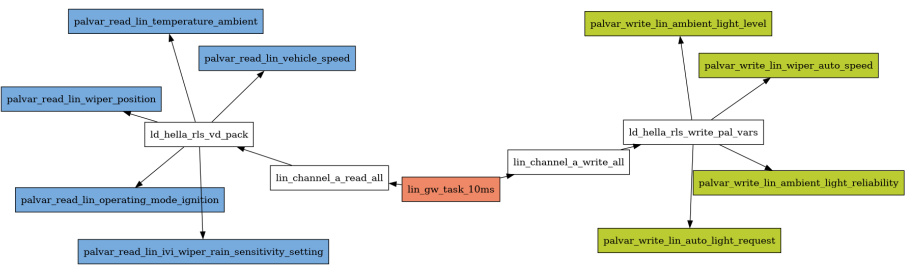
\includegraphics[width=0.9\textwidth]{images/callgraph.png}
    \caption{Example call-graph for the lin\_gw\_task\_10ms runnable}
    \label{fig:callgraph}
\end{figure}

The linker of the LLVM toolchain supports the generation of call-graphs, but only for entire applications or libraries. This means that the resulting call-graph will contain all function calls performed in the programmable end nodes software. LLVM uses the dot language to encode the resulting call-graph, various frameworks exist for processing dot graphs. We have chosen the Networkx python library to extract the required information from the call-graph, the post-process script is available in the projects Github repository. The pseudo-code is shown in listing~\ref{code:pseudo}. The call-graph analysis yields a list of read and write actions, correlated with the runnable executing these actions. As the number of runnables is small, it is easy to find a period per runnable, resulting in a list of read/write rates and source/destination. 

A similar analysis can be performed on the reception and transmission of CAN messages by runnables. As this happens through the real-time operating system's interface, the same call-graph can be searched for \textsc{palcan\_receive} and \textsc{palcan\_transmit} function calls. Unfortunately the CAN receive/transmit function prototypes do not contain relevant information such as CAN bus, message ID or message size. Instead, the function calling the receive/transmit message was recorded together with the runnable name. The required information is then manually recorded through inspection of the calling function. A structured interface description containing the can messages received or transmitted by a runnable would avoid the need for this manual inspection. A different solution would be to generate receive and transmit functions with distinct names for the CAN messages, similar to the data dictionary functions.

The call graph analysis resulted in a database containing 1479 read and write actions of data dictionaries and 616 can messages. From which the \omnet model can be generated.

% \newpage
\lstinputlisting[caption=Call graph analysis pseudocode, label={code:pseudo}, language=Python, firstline=1,frame=single,numbers=left,keywordstyle=\color{blue}]{pseudocode.py}
